\documentclass{standalone}
\usepackage{tikz}
\usetikzlibrary{patterns, positioning}
\usepackage[sfdefault]{ClearSans} %% option 'sfdefault' activates Clear Sans as the default text font
\usepackage[T1]{fontenc}

\begin{document}
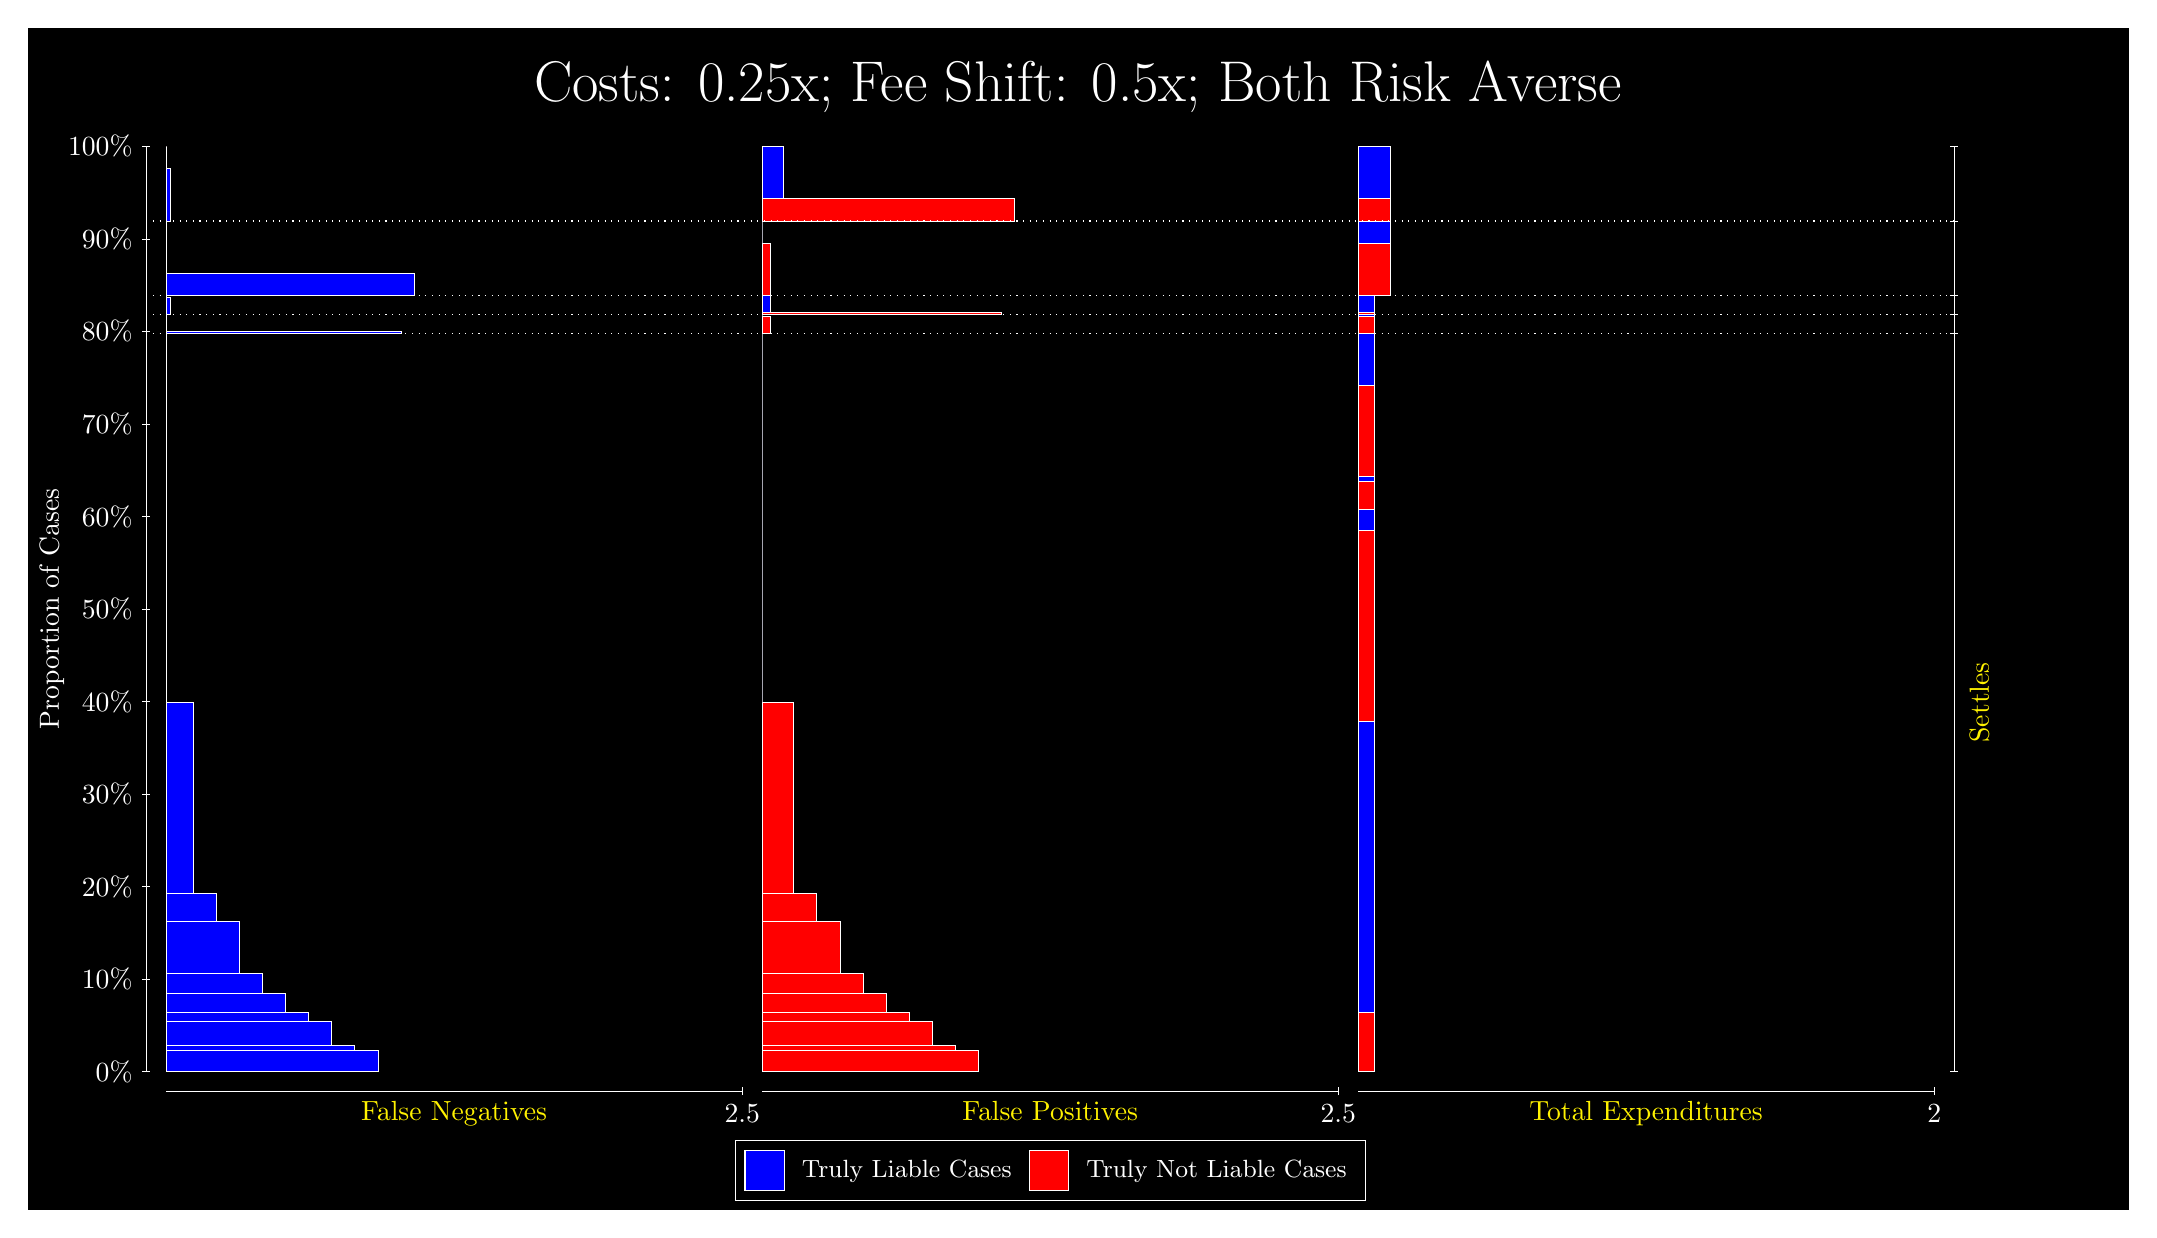
\begin{tikzpicture}
\draw[fill=black] (0,0) rectangle (26.667,15);
\draw[text=white] (0,13.5) rectangle (26.667,15) node[midway] {\huge Costs: 0.25x; Fee Shift: 0.5x; Both Risk Averse};
\draw[white, very thin] (1.5,1.75) -- (1.5,13.5);
\node[rotate=90, text=white, anchor=center] at (0.3, 7.625) {Proportion of Cases};
\draw[white, very thin] (1.45,1.75) -- (1.55,1.75);
\node[text=white, anchor=east] at (1.45, 1.75) {0\%};
\draw[white, very thin] (1.45,2.925) -- (1.55,2.925);
\node[text=white, anchor=east] at (1.45, 2.925) {10\%};
\draw[white, very thin] (1.45,4.1) -- (1.55,4.1);
\node[text=white, anchor=east] at (1.45, 4.1) {20\%};
\draw[white, very thin] (1.45,5.275) -- (1.55,5.275);
\node[text=white, anchor=east] at (1.45, 5.275) {30\%};
\draw[white, very thin] (1.45,6.45) -- (1.55,6.45);
\node[text=white, anchor=east] at (1.45, 6.45) {40\%};
\draw[white, very thin] (1.45,7.625) -- (1.55,7.625);
\node[text=white, anchor=east] at (1.45, 7.625) {50\%};
\draw[white, very thin] (1.45,8.8) -- (1.55,8.8);
\node[text=white, anchor=east] at (1.45, 8.8) {60\%};
\draw[white, very thin] (1.45,9.975) -- (1.55,9.975);
\node[text=white, anchor=east] at (1.45, 9.975) {70\%};
\draw[white, very thin] (1.45,11.15) -- (1.55,11.15);
\node[text=white, anchor=east] at (1.45, 11.15) {80\%};
\draw[white, very thin] (1.45,12.325) -- (1.55,12.325);
\node[text=white, anchor=east] at (1.45, 12.325) {90\%};
\draw[white, very thin] (1.45,13.5) -- (1.55,13.5);
\node[text=white, anchor=east] at (1.45, 13.5) {100\%};

\draw[white, very thin] (24.457,1.75) -- (24.457,13.5);
\draw[white, very thin] (24.407,1.75) -- (24.507,1.75);
\node[anchor=west] at (24.407, 1.75) {};
\draw[white, very thin] (24.407,11.126) -- (24.507,11.126);
\node[anchor=west] at (24.407, 11.126) {};
\draw[white, very thin] (24.407,11.365) -- (24.507,11.365);
\node[anchor=west] at (24.407, 11.365) {};
\draw[white, very thin] (24.407,11.604) -- (24.507,11.604);
\node[anchor=west] at (24.407, 11.604) {};
\draw[white, very thin] (24.407,12.552) -- (24.507,12.552);
\node[anchor=west] at (24.407, 12.552) {};
\draw[white, very thin] (24.407,13.5) -- (24.507,13.5);
\node[anchor=west] at (24.407, 13.5) {};

\draw[white, very thin, fill=blue] (1.75,1.75) rectangle (4.4397,2.0225);
\draw[white, very thin, fill=blue] (1.75,2.0225) rectangle (4.1469,2.085);
\draw[white, very thin, fill=blue] (1.75,2.085) rectangle (3.8542,2.3854);
\draw[white, very thin, fill=blue] (1.75,2.3854) rectangle (3.5614,2.5);
\draw[white, very thin, fill=blue] (1.75,2.5) rectangle (3.2687,2.7405);
\draw[white, very thin, fill=blue] (1.75,2.7405) rectangle (2.9759,3.0035);
\draw[white, very thin, fill=blue] (1.75,3.0035) rectangle (2.6832,3.6629);
\draw[white, very thin, fill=blue] (1.75,3.6629) rectangle (2.3904,4.0182);
\draw[white, very thin, fill=blue] (1.75,4.0182) rectangle (2.0976,6.4381);
\draw[white, very thin, fill=red] (1.75,6.4381) rectangle (1.75,11.126);
\draw[white, very thin, fill=blue] (1.75,11.126) rectangle (4.7324,11.153);
\draw[white, very thin, fill=red] (1.75,11.153) rectangle (1.75,11.365);
\draw[white, very thin, fill=blue] (1.75,11.365) rectangle (1.8049,11.577);
\draw[white, very thin, fill=red] (1.75,11.577) rectangle (1.75,11.604);
\draw[white, very thin, fill=blue] (1.75,11.604) rectangle (4.8971,11.886);
\draw[white, very thin, fill=red] (1.75,11.886) rectangle (1.75,12.552);
\draw[white, very thin, fill=blue] (1.75,12.552) rectangle (1.8049,13.218);
\draw[white, very thin, fill=red] (1.75,13.218) rectangle (1.75,13.5);
\draw[white, very thin, fill=red] (9.3189,1.75) rectangle (12.063,2.0225);
\draw[white, very thin, fill=red] (9.3189,2.0225) rectangle (11.771,2.0849);
\draw[white, very thin, fill=red] (9.3189,2.0849) rectangle (11.478,2.3853);
\draw[white, very thin, fill=red] (9.3189,2.3853) rectangle (11.185,2.5);
\draw[white, very thin, fill=red] (9.3189,2.5) rectangle (10.892,2.7404);
\draw[white, very thin, fill=red] (9.3189,2.7404) rectangle (10.6,3.0035);
\draw[white, very thin, fill=red] (9.3189,3.0035) rectangle (10.307,3.6629);
\draw[white, very thin, fill=red] (9.3189,3.6629) rectangle (10.014,4.0183);
\draw[white, very thin, fill=red] (9.3189,4.0183) rectangle (9.7214,6.4383);
\draw[white, very thin, fill=blue] (9.3189,6.4383) rectangle (9.3189,11.126);
\draw[white, very thin, fill=red] (9.3189,11.126) rectangle (9.4287,11.339);
\draw[white, very thin, fill=blue] (9.3189,11.339) rectangle (9.3189,11.365);
\draw[white, very thin, fill=red] (9.3189,11.365) rectangle (12.356,11.391);
\draw[white, very thin, fill=blue] (9.3189,11.391) rectangle (9.4287,11.604);
\draw[white, very thin, fill=red] (9.3189,11.604) rectangle (9.4287,12.269);
\draw[white, very thin, fill=blue] (9.3189,12.269) rectangle (9.3189,12.552);
\draw[white, very thin, fill=red] (9.3189,12.552) rectangle (12.521,12.834);
\draw[white, very thin, fill=blue] (9.3189,12.834) rectangle (9.5933,13.5);
\draw[white, very thin, fill=red] (16.888,1.75) rectangle (17.094,2.5);
\draw[white, very thin, fill=blue] (16.888,2.5) rectangle (17.094,6.1976);
\draw[white, very thin, fill=red] (16.888,6.1976) rectangle (17.094,8.6176);
\draw[white, very thin, fill=blue] (16.888,8.6176) rectangle (17.094,8.8901);
\draw[white, very thin, fill=red] (16.888,8.8901) rectangle (17.094,9.2455);
\draw[white, very thin, fill=blue] (16.888,9.2455) rectangle (17.094,9.3079);
\draw[white, very thin, fill=red] (16.888,9.3079) rectangle (17.094,10.471);
\draw[white, very thin, fill=blue] (16.888,10.471) rectangle (17.094,11.126);
\draw[white, very thin, fill=red] (16.888,11.126) rectangle (17.094,11.339);
\draw[white, very thin, fill=blue] (16.888,11.339) rectangle (17.094,11.365);
\draw[white, very thin, fill=red] (16.888,11.365) rectangle (17.094,11.391);
\draw[white, very thin, fill=blue] (16.888,11.391) rectangle (17.094,11.604);
\draw[white, very thin, fill=red] (16.888,11.604) rectangle (17.299,12.269);
\draw[white, very thin, fill=blue] (16.888,12.269) rectangle (17.299,12.552);
\draw[white, very thin, fill=red] (16.888,12.552) rectangle (17.299,12.834);
\draw[white, very thin, fill=blue] (16.888,12.834) rectangle (17.299,13.5);
\draw[white, dotted] (1.5,11.126) -- (24.457,11.126);
\draw[white, dotted] (1.5,11.365) -- (24.457,11.365);
\draw[white, dotted] (1.5,11.604) -- (24.457,11.604);
\draw[white, dotted] (1.5,12.552) -- (24.457,12.552);
\draw[white, very thin] (1.75,1.5) -- (9.0689,1.5);
\node[text=yellow, anchor=north] at (5.4094, 1.5) {False Negatives};
\draw[white, very thin] (9.0689,1.45) -- (9.0689,1.55);
\node[text=white, anchor=north] at (9.0689, 1.45) {2.5};

\draw[white, very thin] (9.3189,1.5) -- (16.638,1.5);
\node[text=yellow, anchor=north] at (12.978, 1.5) {False Positives};
\draw[white, very thin] (16.638,1.45) -- (16.638,1.55);
\node[text=white, anchor=north] at (16.638, 1.45) {2.5};

\draw[white, very thin] (16.888,1.5) -- (24.207,1.5);
\node[text=yellow, anchor=north] at (20.547, 1.5) {Total Expenditures};
\draw[white, very thin] (24.207,1.45) -- (24.207,1.55);
\node[text=white, anchor=north] at (24.207, 1.45) {2};

\node[text=yellow, centered, rotate=90] at (24.777, 6.4382) {Settles};





\draw (12.978300999999998,1.5) node[draw=none] (baseCoordinate) {};
\begin{scope}[align=center]
        \matrix[scale=0.5, draw=white, below=0.5cm of baseCoordinate, nodes={draw}, column sep=0.1cm]{
            \node[rectangle, draw, minimum width=0.5cm, minimum height=0.5cm, fill=blue] {}; &
            \node[draw=none, font=\small, text=white] (B) {Truly Liable Cases}; &
            \node[rectangle, draw, minimum width=0.5cm, minimum height=0.5cm, fill=red] {}; &
            \node[draw=none, font=\small, text=white] (B) {Truly Not Liable Cases}; \\
            };
\end{scope}

\end{tikzpicture}
\end{document}